
\documentclass[11pt]{article}
\usepackage[margin=1in]{geometry}
\usepackage{graphicx}
\usepackage{booktabs}
\usepackage{amsmath}
\usepackage{hyperref}
\title{Dense-Angle Two-Moons Benchmark}
\date{}
\begin{document}
\maketitle

\section*{Architecture}
This follow-up benchmark replaces the original 4-qubit HEA with an online-derived two-moons circuit. The adopted structure is the 2-qubit dense-angle classifier used in two-moons tutorials: four trainable input-scaling gates,
\[
R_Y(w_0 x_0),\; R_Y(w_1 x_0),\; R_Z(w_2 x_1),\; R_Z(w_3 x_1),
\]
followed by 4 repeated blocks of
\[
R_Y(\theta_1) R_Y(\theta_2)\,\mathrm{CZ}\,R_Y(\theta_3) R_Y(\theta_4),
\]
and a final pair of $R_Y$ gates measured with $Z_0$. The data preprocessing also follows the centered angle map used in those examples, sending each feature to $[-\pi, \pi]$ on the training split.

\section*{Results}
The optimizer comparison was rerun for Adam, L-BFGS-B, and the best previously discovered hybrid Krotov schedule, with the Krotov step sizes retuned for the new circuit. The aggregate results over 5 seeds are:

\begin{center}
\begin{tabular}{lcccc}
\toprule
Optimizer & Final loss & Test accuracy & Wall time (s) & Time to $L \le 0.40$ (s) \\
\midrule
Hybrid Krotov & 0.346 $\pm$ 0.020 & 0.871 $\pm$ 0.015 & 28.9 $\pm$ 13.0 & 1.22 \\
Adam & 0.344 $\pm$ 0.025 & 0.879 $\pm$ 0.020 & 40.8 $\pm$ 0.1 & 9.35 \\
L-BFGS-B & 0.344 $\pm$ 0.025 & 0.880 $\pm$ 0.019 & 13.3 $\pm$ 3.0 & 4.77 \\
\bottomrule
\end{tabular}
\end{center}

The best mean final loss in this architecture is achieved by \textbf{L-BFGS-B}, although Adam is statistically almost tied. In this corrected rerun, hybrid Krotov reaches mean final loss 0.346 and mean test accuracy 0.871, versus 0.344 / 0.879 for Adam and 0.344 / 0.880 for L-BFGS-B.

The strongest remaining advantage of hybrid Krotov is early progress: it is the fastest method to reach the benchmark threshold $L \le 0.40$, while \textbf{L-BFGS-B} is the fastest optimizer in total wall-clock time. The corrected gradients therefore change the scientific conclusion substantially: the dense-angle architecture does help, but it no longer makes hybrid Krotov dominate the corrected classical baselines.

\section*{Figures}
\begin{center}
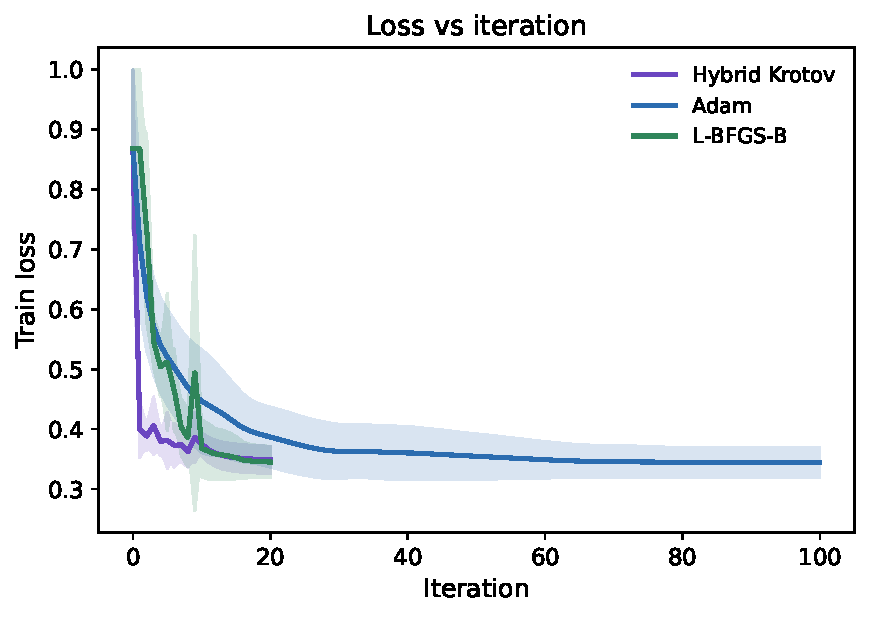
\includegraphics[width=0.78\textwidth]{figures/comparison_loss_vs_iteration.pdf}

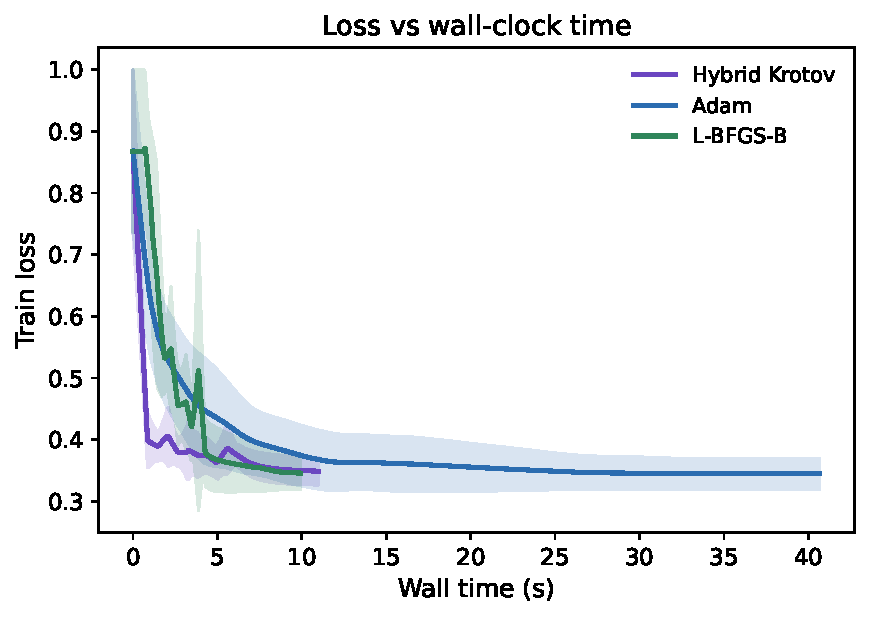
\includegraphics[width=0.78\textwidth]{figures/comparison_loss_vs_time.pdf}

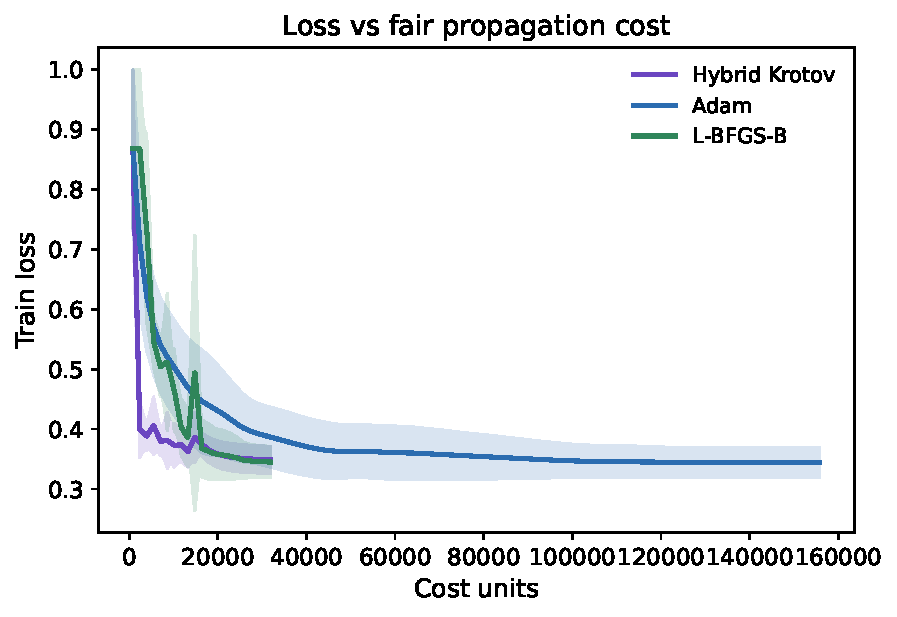
\includegraphics[width=0.78\textwidth]{figures/comparison_loss_vs_cost.pdf}

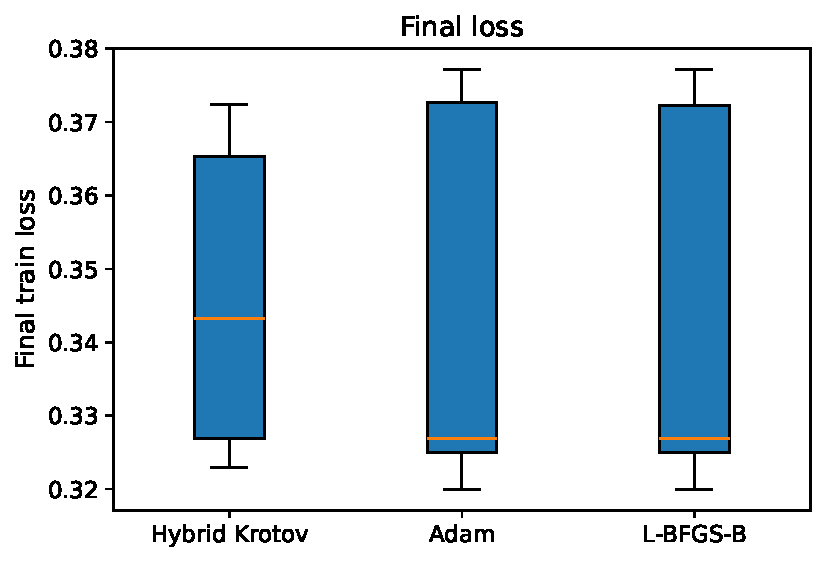
\includegraphics[width=0.62\textwidth]{figures/comparison_final_loss_boxplot.pdf}
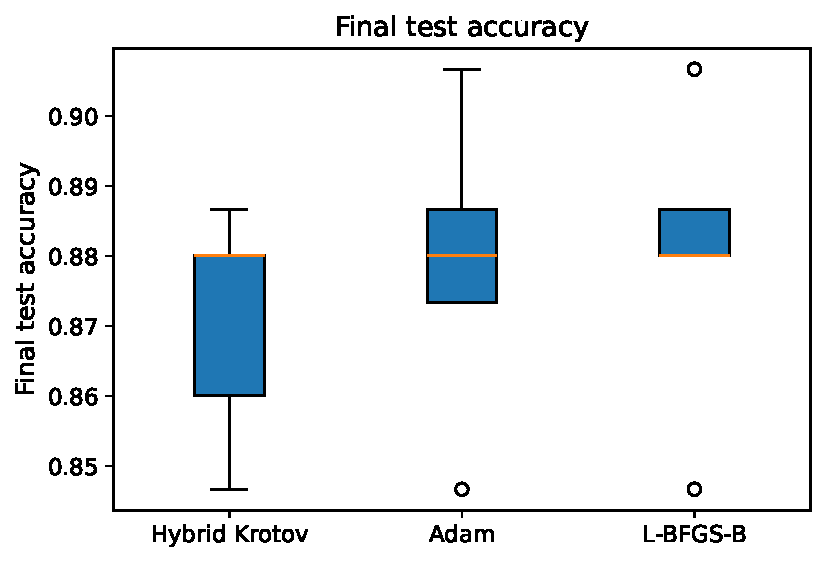
\includegraphics[width=0.62\textwidth]{figures/comparison_final_test_accuracy_boxplot.pdf}

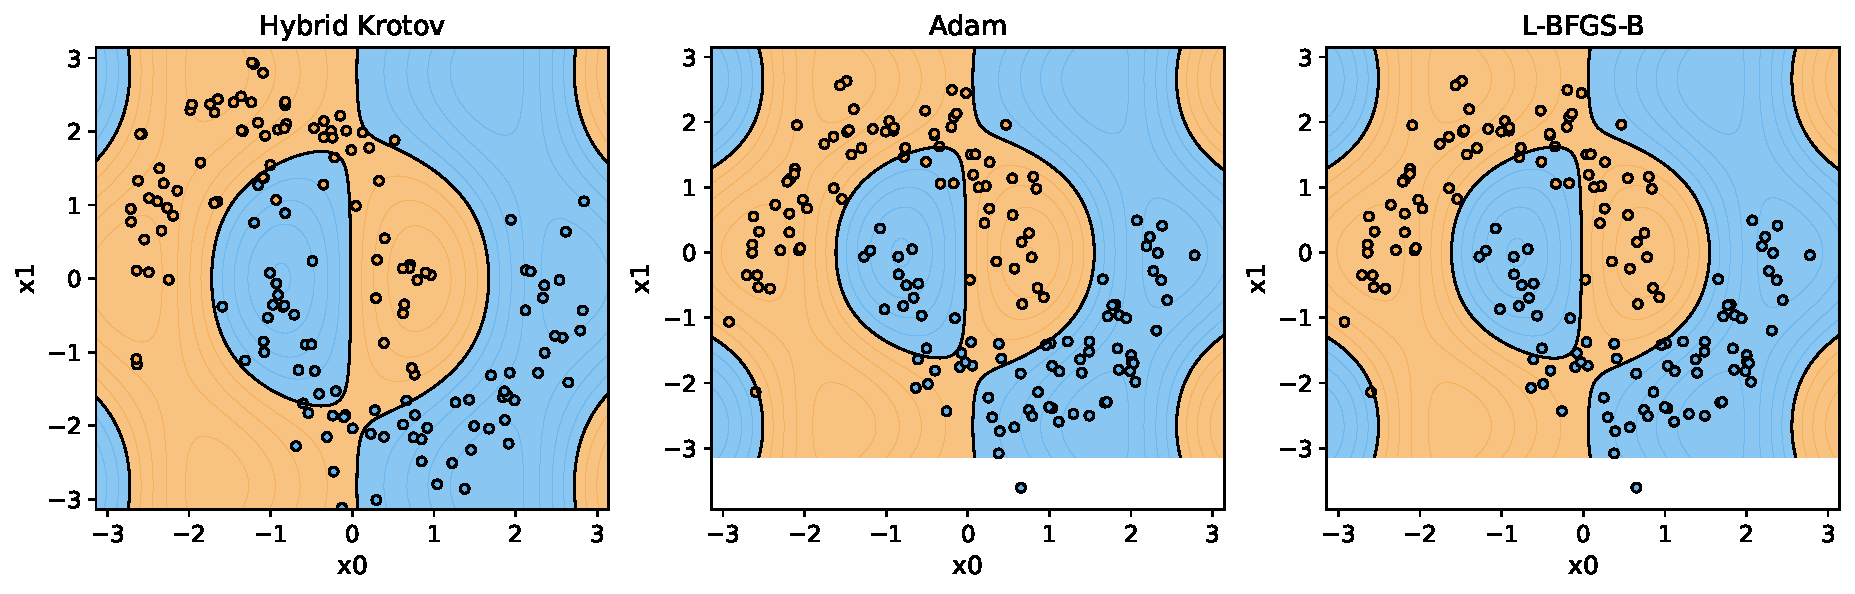
\includegraphics[width=0.92\textwidth]{figures/comparison_decision_boundaries.pdf}
\end{center}

\end{document}
